%-----------------------------------------------------------------------------
%
%               Template for sigplanconf LaTeX Class
%
% Name:         sigplanconf-template.tex
%
% Purpose:      A template for sigplanconf.cls, which is a LaTeX 2e class
%               file for SIGPLAN conference proceedings.
%
% Guide:        Refer to "Author's Guide to the ACM SIGPLAN Class,"
%               sigplanconf-guide.pdf
%
% Author:       Paul C. Anagnostopoulos
%               Windfall Software
%               978 371-2316
%               paul@windfall.com
%
% Created:      15 February 2005
%
%-----------------------------------------------------------------------------


%\documentclass[preprint]{sigplanconf}
\documentclass{article}

% The following \documentclass options may be useful:
%
% 10pt          To set in 10-point type instead of 9-point.
% 11pt          To set in 11-point type instead of 9-point.
% authoryear    To obtain author/year citation style instead of numeric.

\usepackage{yfonts}
\usepackage{amsmath}
\usepackage{amsthm}
\usepackage{amssymb}
%\usepackage{mathpartir}
\usepackage{hyperref}
\usepackage{url}
\usepackage{graphics}
\usepackage{graphicx}
\usepackage{wasysym}
\usepackage{harmony}
\usepackage{marvosym}
\usepackage{multirow}
\usepackage[usenames,dvipsnames]{xcolor}
\usepackage[charter]{mathdesign}
\usepackage{natbib}
\usepackage{xspace}
\usepackage{fullpage}
\usepackage[mathcal]{euscript}
\usepackage[linesnumbered,ruled]{algorithm2e}

\renewcommand{\UrlBreaks}{\do\/\do\a\do\b\do\c\do\d\do\e\do\f\do\g\do\h\do\i\do\j\do\k\do\l\do\m\do\n\do\o\do\p\do\q\do\r\do\s\do\t\do\u\do\v\do\w\do\x\do\y\do\z}

% ____________________________________________________________
% Listings Package Configuration
% \usepackage[scaled]{beramono}

%\renewcommand*\ttdefault{txtt}
\usepackage[T1]{fontenc}

% This Deep Tex Voodoo is from
%   <http://www.latex-community.org/forum/viewtopic.php?f=5&t=2072>
% It's purpose is to make \lstinline normal size, without affecting
% \lstinputlisting.  It seems to work but I have no idea how or why,
% and I rather hope never to learn.
%\makeatletter
%\lst@AddToHook{TextStyle}{\let\lst@basicstyle\ttfamily\normalsize}
%\makeatother

\begin{document}

%\conferenceinfo{SIGBOVIK '18}{Pittsburgh, PA, USA}
%\copyrightyear{2018}
%\copyrightdata{}
%
%\titlebanner{banner above paper title}        % These are ignored unless
%\preprintfooter{short description of paper}   % 'preprint' option specified.

\title{
Transactional Memory Concurrency Verification with Landslide
%That `Boring' Stuff Was Part of the Title, BTW. \\
%So was that. And that, and this too. \\
%You got it all, right? \\
%Or Just, ``More Boring Crap about ITG'', for Short. \\
%Oh, That Was Also Part of the Title.
}
% \subtitle{\em The Randomly-Scoped Lambda Calculus}
% \subtitle{Subtitle Text, if any}

\author{Ben Blum \\ bblum@cs.cmu.edu}
\date{}

\maketitle

%\category{D.1.3}{Programming Techniques}{Concurrent Programming}
%\category{D.2.4}{Software Engineering}{Software/Program Verification}
%
%\keywords
%landslide terminal, baggage claim, ground transportation, ticketing


\section{Background}
\label{sec:background}

\subsection{Hardware transactional memory}

Transactional Synchronization Extensions (TSX) was implemented on consumer hardware for the first time by Intel's Haswell architecture \cite{htm-haswell},
which extends the x86 instruction set to provide
{\tt xbegin}, {\tt xend}, and {\tt xabort} for beginning, committing, and aborting
transactions, respectively.
Higher-level programming languages or compilers may offer libraries or intrinsics to access these instructions;
for C and C++ GCC provides intrinsics named {\tt \_xbegin()} and so on \cite{htm-gcc}.
Figure~\ref{fig:htm-example} shows an example program using TSX to synchronize access to a shared counter,
including a failure path which defaults to a conventional lock.
%This example actually has a bug, which we will discuss in the next section;
%the reader is encouraged to try to spot it before then.
Several related works formally prove the correctness of transactional memory {\em implementations}
\cite{specifying-verifying-tm,tm-correctness,tm-completeness,mc-tm-with-spin},
but verifying the client programs written to use transactions remains an open problem.

\newcommand\hilight[2]{\color{#1}#2\color{black}}
\definecolor{orange}{RGB}{192,96,0}
\definecolor{olivegreen}{RGB}{0,127,0}
\definecolor{brickred}{RGB}{192,0,0}
\definecolor{commentblue}{RGB}{0,0,192}
\definecolor{black}{RGB}{0,0,0}
%\definecolor{lavender}{RGB}{238,85,238}
%\definecolor{seafoam}{RGB}{85,238,102}
%\definecolor{salmon}{RGB}{238,102,85} % ee6655

% threads
\definecolor{lavender}{RGB}{102,65,208} % (?? i don't know what happened here anymore but it looks good)
\definecolor{seafoam}{RGB}{56,158,68} % * 2/3
\definecolor{salmon}{RGB}{208,89,74} % * 7/8

% eval data
\definecolor{darkcyan}{RGB}{0,128,128}
\definecolor{lime}{RGB}{48,128,0}
\definecolor{darklavender}{RGB}{68,44,138}
\definecolor{brownish}{RGB}{128,96,0}
\definecolor{pinkish}{RGB}{128,34,102} % ff4488

% syntax hilighting
\definecolor{brown}{RGB}{170,85,0}
% \definecolor{pink}{RGB}{170,45,136} % pinkish * 4/3 % but actually looks better darker
\newcommand\flow[1]{\hilight{brown}{#1}\xspace}
\newcommand\const[1]{\hilight{brickred}{#1}\xspace}
\newcommand\call[1]{\hilight{pinkish}{#1}}

Under software transactional memory (STM) \cite{stm-pldi06},
memory conflicts with other threads are the only reason for transaction failure
(apart from programmer-supplied explicit aborts);
hence, depending on program semantics, some transactions may be guaranteed to succeed.
However, hardware transactions (HTM) may also fail
for several other reasons such as random system interrupts or exhausting the CPU's cache capacity.
Because timer interrupts can in principle occur at any moment,
and with arbitrary frequency (observable by the program, perhaps as a result of a heavily-loaded system),
in this paper we will simplify the failure model by saying that HTM transactions can fail for any reason.
%We defer discussion of programs which distinguish the reason for aborts through the failure code to Section~\ref{sec:warpzone}.

\subsection{Stateless model checking}

Model checking (MC) \cite{verisoft} is a testing technique for systematically executing and verifying
the possible thread interleavings of a concurrent program.
The main research challenge is to cope with exponential explosion of the state space,
which is sized $O(n^k)$ for a program with $n$ operations and $k$ threads.
Some {\em stateful} MCs explicitly store and compare all visited states of the program being tested \cite{spin},
which both keeps track of test coverage
and allows identifying identical states to avoid testing redundant interleavings.
%
By contrast, {\em stateless} MC (henceforth abbreviated simply as MC)
stores only the current sequence of execution events to avoid a prohibitive memory footprint.
Reduction algorithms \cite{dpor,optimal-dpor,satcheck,mcr,mcr,tsopso}
can then analyze the memory accesses in that sequence to identify
interleavings observationally-equivalent under Mazurkiewicz trace theory \cite{mazurkiewicz} and hence safe to skip.
The resulting state spaces are still exponentially-sized,
but only in the number of conflicting operations rather than all operations.
%Of these, Landslide uses Dynamic Partial Order Reduction (DPOR) \cite{dpor} to prune its state spaces.

\begin{figure}[t]
	\begin{center}
		\begin{tabular}{ll}
		%\texttt{void count() \{} \\
		%\texttt{~~~~for (int i = 0; i < 1000; i++) \{} \\
		1 & \texttt{\flow{if} (\call{\_xbegin}() == \const{SUCCESS}) \{} \\
		2 & \texttt{~~~~x++;} \\
		3 & \texttt{~~~~\call{\_xend}();} \\
		4 & \texttt{\} \flow{else} \{} \\
		5 & \texttt{~~~~\call{mutex\_lock}(\&m);} \\
		6 & \texttt{~~~~x++;} \\
		7 & \texttt{~~~~\call{mutex\_unlock}(\&m);} \\
		8 & \texttt{\}} \\
		%\texttt{~~~~\}} \\
		%\texttt{\}} \\
		\end{tabular}
	\end{center}
	\caption{Example transactional programs.
			If the
			%transaction in the
			top branch aborts,
			%whether from a memory conflict or random system interrupt,
			%from the programmer's intention,
			execution will revert to the return of {\tt \_xbegin()}
			%{\tt status} will be assigned an error code
			and control will drop into the {\tt else} branch.
			The programmer can then use explicit synchronization
			%, such as a mutex,
			to resolve the conflict.
		}
	\label{fig:htm-example}
\end{figure}
MCs may instrument programs to introduce thread switches at varying granularity, which affects the number of operations $n$.
%The number of operations depends on how finely-grained the MC instruments the program to introduce thread switches.
Some target distributed systems, instrumenting only message-passing events \cite{modist};
some run multithreaded programs natively, instrumenting only the pthread API for performance \cite{dbug-ssv};
and some insert compiler instrumentation on statically-identified memory accesses \cite{chess,inspect}.
Our model checker, Landslide \cite{landslide},
traces every memory access through the use of a simulated environment \cite{bochs},
which is important for identifying data races to use as new preemption points \cite{quicksand},
as well as for identifying when a memory conflict may cause transaction aborts.
With regard to checking for bugs,
the ``model'' the name refers to being checked may be
an external formal specification,
the program's own internal consistency checks,
or a set of expected properties encoded in the tool itself.
Landslide uses the latter two cases, checking for assertion failures
as well as deadlocks, use-after-frees, and segfaults.
%For this work we also detect use of {\tt xend} outside of a transaction
%or {\tt xbegin} within one as a bug.

\subsection{Example bug}
\label{sec:example}

\newcommand\tii{\ensuremath{\hilight{lavender}{\mathbf{Ti}}}\xspace}
\newcommand\tjj{\ensuremath{\hilight{seafoam}{\mathbf{Tj}}}\xspace}
\newcommand\tkk{\ensuremath{\hilight{salmon}{\mathbf{Tk}}}\xspace}

\newcommand\tiiat[1]{\ensuremath{\hilight{lavender}{\mathbf{Ti}@#1}}\xspace}
\newcommand\tjjat[1]{\ensuremath{\hilight{seafoam} {\mathbf{Tj}@#1}}\xspace}
\newcommand\tkkat[1]{\ensuremath{\hilight{salmon}  {\mathbf{Tk}@#1}}\xspace}

Consider again the program in Figure~\ref{fig:htm-example}.
Note that the C-style {\tt x++} operations, when compiled into assembly.
results in multiple memory accesses which can be interleaved with other threads.
\[
\begin{tabular}{ll}
	$2a$ & \texttt{temp <- x;} \\
	$2b$ & \texttt{temp <- temp + 1;} \\
	$2c$ & \texttt{x <- temp;} \\
\end{tabular}
\]

The {\tt x++} operation from the failure path
%(correspondingly $6a$, $6b$, $6c$)
can by interrupted with conflicting accesses from the transaction path interleaved in between,
since the mutex only protects the failure path against other failure paths,
but not against the transaction itself.
Hence an interleaving such as the following is possible,
in which only two increments of {\tt x} are observed while three are expected.

\[
\begin{tabular}{ll|ll|ll}
	\multicolumn{2}{c|}{\hilight{lavender}{\bf Thread 1}} &
	\multicolumn{2}{c|}{\hilight{seafoam}{\bf Thread 2}} &
	\multicolumn{2}{c}{\hilight{salmon}{\bf Thread 3}} \\
	\hline
	\hilight{lavender}{$1$} & \hilight{lavender}{\texttt{\_xbegin();}} & & \\
	%
	& & \hilight{seafoam}{$1$} & \hilight{seafoam}{\texttt{\_xbegin();}} \\
	& & \hilight{seafoam}{$2$} & \hilight{seafoam}{\texttt{x++;}} \\
	& & \hilight{seafoam}{$3$} & \hilight{seafoam}{\texttt{\_xend();}} \\
	%
	& \hilight{lavender}{\em transaction fails} & & & \\
	\hilight{lavender}{$5$} & \hilight{lavender}{\texttt{mutex\_lock(m);}} & & \\
	\hilight{lavender}{$6a$} & \hilight{lavender}{\texttt{temp <- x;}} & & \\
	%
	& & & & \hilight{salmon}{$1$} & \hilight{salmon}{\texttt{\_xbegin();}} \\
	& & & & \hilight{salmon}{$2$} & \hilight{salmon}{\texttt{x++;}} \\
	& & & & \hilight{salmon}{$3$} & \hilight{salmon}{\texttt{\_xend();}} \\
	%
	\hilight{lavender}{$6b$} & \hilight{lavender}{\texttt{temp <- temp + 1;}} & & \\
	\hilight{lavender}{$6c$} & \hilight{lavender}{\texttt{x <- temp;}} & & \\
	\hilight{lavender}{$7$} & \hilight{lavender}{\texttt{mutex\_unlock(m);}} & & \\
\end{tabular}
\]


Prior work \cite{htm-mario} proposed the idiom shown in Figure~\ref{fig:htm-fixed}
to exclude interleavings which violate the failure path's atomicity such as shown above.
Thread 1 would set the {\tt prevent\_transactions} flag across its {\tt x++} accesses,
and
Thread 3 would have to check it and trigger an abort. %(Figure \ref{fig:htm-fixed} lines 2-3).
%which shows that correctly synchronizing even the simplest transactions may be surprisingly difficult or complex.
%further motivating our research.

\begin{figure}[t]
	\begin{center}
		\begin{tabular}{ll}
			%\texttt{void count() \{} \\
			%\texttt{~~~~for (int i = 0; i < 1000; i++) \{} \\
			  & \texttt{prevent\_transactions = \const{false};} \\
			\\
			0 & \texttt{\flow{while} (prevent\_transactions) \flow{continue};} \\
			1 & \texttt{\flow{if} (\call{\_xbegin}() == \const{SUCCESS}) \{} \\
			2 & \texttt{~~~~\flow{if} (prevent\_transactions)} \\
			3 & \texttt{~~~~~~~~\call{\_xabort}();} \\
			4 & \texttt{~~~~x++;} \\
			5 & \texttt{~~~~\call{\_xend}();} \\
			6 & \texttt{\} \flow{else} \{} \\
			7 & \texttt{~~~~\call{mutex\_lock}(\&m);} \\
			8 & \texttt{~~~~prevent\_transactions = \const{true};} \\
			9 & \texttt{~~~~x++;} \\
			A & \texttt{~~~~prevent\_transactions = \const{false};} \\
			B & \texttt{~~~~\call{mutex\_unlock}(\&m);} \\
			C & \texttt{\}} \\
		\end{tabular}
	\end{center}
	\caption{Variant %of the program in Figure~\ref{fig:htm-example},
		with additional synchronization to protect the failure path from the transactional path.
		The optional line 0 serves to prevent a cascade of failure paths
		for the sake of performance
		by allowing threads to wait until transacting is safe again.
		}
	\label{fig:htm-fixed}
\end{figure}


%%%%%%%%%%%%%%%%%%%%%%%%%%%%%%%%%%%%%%%%%%%%%%%%%%%%%%%%%%%%%%%%%%%%%%%%%%%%%%%%

\newpage
\section{Implementation}

To model check a transactional program it suffices to test a set of interleavings
corresponding to all {\em observable} behaviours of the program.
Because incomplete transactions are rolled back upon abort,
we claim that interleaving other threads within the body of a transaction is never necessary,
and hence model checking can achieve full coverage simply by conisdering each {\tt xbegin} invocation
to be a preemption point with nondeterministic failure injection.
Appendix~\ref{sec:proofs} provides several proof sketches to justify this claim.

Our implementation of HTM-equivalent semantics has been incorporated by the Landslide maintainers upstream.
It is available open-source at \url{https://github.com/bblum/landslide}.
Programs should be ported to the Pebbles userland \cite{thrlib,kspec},
their use of compiler HTM intrinsics should be replaced with the Landslide stubs provided in {\tt 410user/inc/htm.h},
and HTM nondeterminism can then be enabled with the {\tt -X} command-line flag.
%We have also extended its Iterative Deepening implementation \cite{quicksand}
%with a new option ({\tt -M} flag) to
%to optimize for completion time by prioritizing the maximal state space job and cancelling all others
%(which maintains its soundness guarantee)
%which we will use in our evaluation.
%All test cases therein are also available in the repository linked above.
All test cases in our evaluation to follow are also available in the repository linked above.

%%%%%%%%%%%%%%%%%%%%%%%%%%%%%%%%%%%%%%%%%%%%%%%%%%%%%%%%%%%%%%%%%%%%%%%%%%%%%%%%

\section{Evaluation}

\newcommand\ETA[1]{\hilight{brownish}{{\em #1}}\xspace}
\newcommand\cpu[1]{\hilight{darkcyan}{{#1}}\xspace}
\newcommand\wtm[1]{\hilight{lime}{{#1}}\xspace}
\newcommand\ints[1]{\hilight{pinkish}{{#1}}\xspace}

%To the best of our knowledge, this is the first work to test transactional programs in a model-checking environment,
%%To the best of the author's knowledge, Landslide is the first MC to check transactional concurrency,
%so no other MC State of the Art%
%\footnote{The author's DJ name.}
%exists to compare to in controlled experiments.
%Nevertheless, we pose the following evaluation questions.

%\begin{enumerate}
%	\item How quickly does Landslide find bugs in incorrect transactional programs of varying sizes?
%	\item How quickly does Landslide verify correct transactional programs of varying sizes?
%	%\item Does Landslide find any previously-unknown bugs in real-world transactional code?
%	\item By the way, should MC research papers quantify variance in their CPU-time performance experiments?
%\end{enumerate}

Our preliminary evaluation evaluates Landslide's bug-finding performance on tests with subtle concurrency errors,
as well as its verification performance on (as far as we know) correct tests.
So far we have several hand-written unit tests
and \cite{htm-mario}'s microbenchmarks and transactional AVL tree and separate-chaining hashmap,
as follows.

\begin{itemize}
	\item {\tt htm1}: The bug from Figure~\ref{fig:htm-example}. %(assertion failure on {\tt count}).
	\item {\tt htm2}: The fixed version as in Figure~\ref{fig:htm-fixed}.
	\item {\tt counter}: Microbenchmark version of {\tt htm2} which replaces the complex failure path with a simple {\tt xadd}.
	\item {\tt swap}: Microbenchmark that swaps values in an array.
	\item {\tt swapbug}: {\tt swap} modified to introduce circular locking in the failure path. %(deadlock).
	\item {\tt avl\_insert}: AVL tree concurrent insertion test.
	\item {\tt avl\_fixed}: {\tt avl\_insert} with the AVL bug fixed. %(spoilers!!).
	\item {\tt map\_basic}: Separate-chaining hashmap concurrent insertion test.
	\item {\tt map\_basicer}: {\tt map\_basic} modified with a larger initial size to skip the resizing step.
\end{itemize}

The notation {\tt testname}$(K,N)$ will denote a test configuration of $K$ threads, each running $N$ iterations of the test logic.
All tests were run on an 8-core 2.7GHz Core i7 with 32 GB RAM.

\subsection{Bugs}
\label{sec:bugs}

Table~\ref{tab:buges}
presents our bug-finding results.
%We configured Landslide to run the Quicksand algorithm \cite{quicksand}
%% this note obsolete since swapbug was fixed and ends at 3,2
%%\footnote{This was necessary in {\tt swapbug}s (4,1) and (4,2) to trigger a switch to the buggy state space.}
%shown left,
%as well as to prioritize the maximal state space as discussed above,
%shown right,
%each with a time limit of 30 minutes.
%
Most notably,
in addition to the bugs we intentionally wrote in {\tt htm1} and {\tt swapbug},
to our pleasant surprise
Landslide also found a previously-unknown bug in the transactional AVL tree,
exposed by {\tt avl\_insert} with any parameters higher than (2,1).
Figure~\ref{fig:avlbug} shows the root cause, essentially the {\tt htm1} bug in disguise.
% landslide-trace-1521093835.18927.html
This manifested
alternately
%in (2,2) and (3,1)
as a segfault
% landslide-trace-1521092404.23772.html
and
%in (2,3)
as a consistency-check assertion failure.
The presence of {\tt while (\_retry);} makes the necessary preemption window extremely small
in practice (between it and {\tt \_xbegin()}),
whereas MC is blind to such matters of chance.%
% NB. In case a reader doesn't believe this footnote,
% I put the loop back in (with thr_yield(-1) therein) to restore the original state space,
% and found the bug with these statistics:
% [JOB 28] progress: 1957/3005897 brs (0.065105%), ETA 6414673y 121d 18h 28m 59s (elapsed 3m 15s)
% [JOB 28] BUG FOUND: landslide-trace-1521099044.76395.html (1958 interleavings tested; 3 preemptions; job time 3m 15s; pldi time 746832861; new-fixed pldi cputime 823243872)
%\footnote{Considering the loop does not affect the test's possible behaviours,
%only its {\em likely} ones,
%we removed it in Landslide's version of the test to keep the state space size manageable.}
%We removed the loop in Landslide's version of the test
%%To make this test Landslide-friendly, we removed that loop,
%which reduces the state space size, but maintains the program's semantics.}
The fact that even Figure~\ref{fig:htm-fixed}'s protocol's very proposer % こそさえ
didn't get it right every time %motivates the need for MC on such programs,
%and perhaps also means TSX primitives should be used only behind higher-level abstractions
%such as lock elision \cite{lock-elision}.
%and
suggests TSX primitives should be encapsulated behind higher-level abstractions
such as lock elision \cite{lock-elision},
which can be verified in isolation with smaller state spaces
then trusted in turn when checking their client programs \cite{dbug-phdthesis}.

\begin{table*}[h]
	\begin{center}
	\begin{tabular}{cc||r|r|r|r}
		\bf buggy test	& \bf params&\cpu{\bf cpu (s)}&\wtm{\bf wall (s)}&\ints{\bf int's}& \ETA{\bf SS size (est.)} \\
		\hline
		\hline
		{\tt htm1}
			& 2,1	&\cpu{*9.47}& \wtm{*6.40}& \ints{21	}& \ETA{213} \\
		(assertion)
			& 2,2	&\cpu{*10.39}& \wtm{*7.70}& \ints{49	}& \ETA{1536} \\
			& 2,3	&\cpu{*12.83}& \wtm{*9.67}& \ints{113	}& \ETA{10752} \\
			& 2,4	&\cpu{*18.63}& \wtm{*15.86}& \ints{257	}& \ETA{73728} \\
		\cline{2-6}
			& 3,1	&\cpu{*9.50}& \wtm{*6.79}& \ints{21	}& \ETA{13653} \\
			& 3,2	&\cpu{*10.72}& \wtm{*7.97}& \ints{49	}& \ETA{393216} \\
			& 3,3	&\cpu{*13.84}& \wtm{*11.01}& \ints{113	}& \ETA{11010048} \\
			& 3,4	&\cpu{*31.37}& \wtm{*28.53}& \ints{257	}& \ETA{301989888} \\
		\cline{2-6}
			& 4,1	&\cpu{*9.82}& \wtm{*7.00}& \ints{21	}& \ETA{873813} \\
			& 4,2	&\cpu{*11.54}& \wtm{*8.55}& \ints{49	}& \ETA{100663296} \\
		\hline
		{\tt swapbug}
			& 2,1	&\cpu{*38.96}& \wtm{*13.15}& \ints{109	}& \ETA{194} \\
		(deadlock)
			& 2,2	&\cpu{*44.73}& \wtm{19.47}& \ints{281	}& \ETA{1620} \\
			& 2,3	&\cpu{*60.30}& \wtm{*35.55}& \ints{718	}& \ETA{12748} \\
			& 2,4	&\cpu{*108.58}& \wtm{82.60}& \ints{1820	}& \ETA{97823} \\
		\cline{2-6}
			& 3,1	&\ETA{--}&\ETA{>30m}&\ETA{--}& \ETA{184984} \\
			& 3,2	&\ETA{--}&\ETA{>30m}&\ETA{--}& \ETA{3099225} \\
		\hline
		{\tt avl\_insert}
			& 2,2	&\cpu{*81.00}&\wtm{*40.30}&\ints{336}&\ETA{379982} \\
		(segfault+)
			& 2,3	&\cpu{*1331.79}&\wtm{1274.36}&\ints{13926}&\ETA{96248131} \\
			& 2,4	&\ETA{--}&\ETA{>30m}&\ETA{--}& \ETA{36019973} \\
		\cline{2-6}
			& 3,1	&\cpu{*69.99}&\wtm{*24.25}&\ints{78}&\ETA{1572107} \\
			& 3,2	&\ETA{--}&\ETA{>30m}&\ETA{--}& \ETA{1402363529} \\
	\end{tabular}
	\end{center}
	\caption{Landslide's bug-finding performance on various test configurations.
		A parameter of $K,N$ denotes $K$ threads each running the test logic for $N$ iterations.
		We list the CPU-time and wall-clock time %(both in seconds)
		elapsed, %until the bug was found,
		plus the number of interleavings of the ultimately buggy state space tested,
		before the bug was found.
		Lastly, Landslide's state space size estimation \cite{estimation},
		though approximate at best,
		confers a sense of the exponential explosion.
	}
	\label{tab:buges}
\end{table*}
%\begin{table*}[t]
%	\begin{center}
%	\begin{tabular}{cc||r|r|r||r|r|r|r}
%			&	&\multicolumn{3}{c||}{\bf Quicksand mode}&\multicolumn{4}{c}{{\bf Maximal state space mode} ({\tt -M})} \\
%		\bf buggy test	& \bf params&\cpu{\bf cpu (s)}&\wtm{\bf wall (s)}&\ints{\bf int's}&\cpu{\bf cpu (s)}&\wtm{\bf wall (s)}&\ints{\bf int's}& \ETA{\bf SS size (est.)} \\
%		\hline
%		\hline
%		{\tt htm1}
%			& 2,1	&\cpu{  45.78}&\wtm{9.70}&\ints{21}& \cpu{*9.47}& \wtm{*6.40}& \ints{21	}& \ETA{213} \\
%		(assertion)
%			& 2,2	&\cpu{  84.14}&\wtm{13.59}&\ints{*33}& \cpu{*10.39}& \wtm{*7.70}& \ints{49	}& \ETA{1536} \\
%			& 2,3	&\cpu{ 131.91}&\wtm{20.44}&\ints{*73}& \cpu{*12.83}& \wtm{*9.67}& \ints{113	}& \ETA{10752} \\
%			& 2,4	&\cpu{ 255.75}&\wtm{37.56}&\ints{257}& \cpu{*18.63}& \wtm{*15.86}& \ints{257	}& \ETA{73728} \\
%		\cline{2-9}
%			& 3,1	&\cpu{ 114.06}&\wtm{17.45}&\ints{*15}& \cpu{*9.50}& \wtm{*6.79}& \ints{21	}& \ETA{13653} \\
%			& 3,2	&\cpu{ 109.60}&\wtm{26.16}&\ints{49}& \cpu{*10.72}& \wtm{*7.97}& \ints{49	}& \ETA{393216} \\
%			& 3,3	&\cpu{ 124.80}&\wtm{20.40}&\ints{*73}& \cpu{*13.84}& \wtm{*11.01}& \ints{113	}& \ETA{11010048} \\
%			& 3,4	&\cpu{ 227.49}&\wtm{35.15}&\ints{*161}& \cpu{*31.37}& \wtm{*28.53}& \ints{257	}& \ETA{301989888} \\
%		\cline{2-9}
%			& 4,1	&\cpu{ 53.08}&\wtm{9.79}&\ints{*15}& \cpu{*9.82}& \wtm{*7.00}& \ints{21	}& \ETA{873813} \\
%			& 4,2	&\cpu{117.07}&\wtm{19.09}&\ints{*33}& \cpu{*11.54}& \wtm{*8.55}& \ints{49	}& \ETA{100663296} \\
%		\hline
%		{\tt swapbug}
%			& 2,1	&\cpu{ 70.95}&\wtm{13.45}&\ints{*16}& \cpu{*38.96}& \wtm{*13.15}& \ints{109	}& \ETA{194} \\
%		(deadlock)
%			& 2,2	&\cpu{ 107.28}&\wtm{*17.45}&\ints{*146}& \cpu{*44.73}& \wtm{19.47}& \ints{281	}& \ETA{1620} \\
%			& 2,3	&\cpu{ 280.05}&\wtm{38.70}&\ints{*352}& \cpu{*60.30}& \wtm{*35.55}& \ints{718	}& \ETA{12748} \\
%			& 2,4	&\cpu{ 617.94}&\wtm{*81.50}&\ints{*834}& \cpu{*108.58}& \wtm{82.60}& \ints{1820	}& \ETA{97823} \\
%		\cline{2-9}
%			& 3,1	&\cpu{*1275.04}&\wtm{*163.42}&\ints{*771}&\ETA{--}&\ETA{>30m}&\ETA{--}& \ETA{184984} \\
%			& 3,2	&\ETA{--}&\ETA{>30m}&\ETA{--}&\ETA{--}&\ETA{>30m}&\ETA{--}& \ETA{3099225} \\
%		% whoops, this was with the dumb lock ordering
%		%	& 3,1	& 11.19	& 3.46	& 9	& 3.13	& 3.13	& 9	& 432 \\
%		%	& 3,2	& 12.41	& 3.76	& 19	& 3.33	& 3.33	& 19	& 5832 \\
%		%	& 3,3	& 15.77	& 4.58	& 41	& 3.95	& 3.95	& 41	& 77759 \\
%		%	& 3,4	& 24.82	& 6.85	& 89	& 5.20	& 5.20	& 89	& 1026431 \\
%		%\cline{2-9}
%		%	& 4,1	& 702.33& 98.06	& 361	& 90.94	& 64.27	& 1607	& 138758 \\
%		%	& 4,2	&9738.43&1257.20& 3023	& 674.87& 650.58& 16511	& 13755188 \\
%		\hline
%		{\tt avl\_insert}
%			& 2,2	&\cpu{488.07}&\wtm{64.77}&\ints{*83}	&\cpu{*81.00}&\wtm{*40.30}&\ints{336}&\ETA{379982} \\
%		(segfault+)
%			% XXX: this 2,3 -M-mode bug was found *mostly* running in isolation,
%			% but for the last few minutes i had another landslide running in parallel bc i thought itd time out.
%			% according to variance expt, it should be rerun for a *minor* speedup, but i can't be bothered
%			& 2,3	&\cpu{2670.87}&\wtm{*330.45}&\ints{*3066}&\cpu{*1331.79}&\wtm{1274.36}&\ints{13926}&\ETA{96248131} \\
%			& 2,4	&\cpu{*3259.37}&\wtm{*436.50}&\ints{*1639}&\ETA{--}&\ETA{>30m}&\ETA{--}& \ETA{36019973} \\
%			% smaller than above? estimate's just fickle i guess; they can go up or down with time
%		\cline{2-9}
%			& 3,1	&\cpu{222.02}&\wtm{40.04}&\ints{*28}	&\cpu{*69.99}&\wtm{*24.25}&\ints{78}&\ETA{1572107} \\
%			& 3,2	&\cpu{*1569.09}&\wtm{*216.85}&\ints{*209}&\ETA{--}&\ETA{>30m}&\ETA{--}& \ETA{1402363529} \\
%	\end{tabular}
%	\end{center}
%	\caption{Landslide's bug-finding performance on various test configurations.
%		Quicksand's workqueue approach optimized for fast bug-finding
%		is compared against our maximum-state-space-prioritizing approach for fast verification.
%		For each, we list the CPU-time and wall-clock time %(both in seconds)
%		elapsed, %until the bug was found,
%		plus the number of interleavings of the ultimately buggy state space tested,
%		before the bug was found.
%		* marks the winning measurements between each series.
%		Lastly, Landslide's state space size estimation \cite{estimation},
%		though approximate at best,
%		confers a sense of the exponential explosion.
%	}
%	\label{tab:buges}
%\end{table*}

\begin{figure}[t]
	\begin{center}
		\begin{tabular}{l}
		%\texttt{void count() \{} \\
		%\texttt{~~~~for (int i = 0; i < 1000; i++) \{} \\
		\texttt{\flow{while} (\_retry);} \\
		\texttt{\flow{if} (\call{\_xbegin}() == \const{SUCCESS}) \{} \\
		\texttt{~~~~\hilight{brickred}{tie}(\_root,inserted) = \call{\_insert}(\_root,n); } \\
		\texttt{~~~~\call{\_xend}();} \\
		\texttt{\} \flow{else} \{} \\
		\texttt{~~~~\call{pthread\_mutex\_lock}(\&\_tree\_lock);} \\
		\texttt{~~~~\_retry = \const{true};} \\
		\texttt{~~~~\hilight{brickred}{tie}(\_root,inserted) = \call{\_insert}(\_root,n); } \\
		\texttt{~~~~\_retry = \const{false};} \\
		\texttt{~~~~\call{pthread\_mutex\_unlock}(\&\_tree\_lock);} \\
		\texttt{\}} \\
		\end{tabular}
	\end{center}
	%\caption{mario man had a very large house. or a castle.}
	\caption{Unmodified code from {\tt htmavl.hpp} showing the previously-unknown bug found by Landslide.
		The transaction path fails to check {\tt \_retry},
		leading to data races and corruption just as in {\tt htm1}.
		}
	\label{fig:avlbug}
\end{figure}

\newpage
\subsection{Verification}

Landslide proved several of our test configurations correct, as shown in Table~\ref{tab:verifs}
%With no bugs to find, comparing the different testing modes against each other is meaningless;
%we simply present their state space sizes and runtime (using {\tt -M}) in Table~\ref{tab:verifs}.
Several larger tests we were unable to complete. %within several hours.
% バレちゃった
%before the submission deadline are also shown.
%Their completion times are listed as {\em unk.}
These are indicated with $\dagger$ %\ETAdag{}
and their listed ETAs and state space sizes represent Landslide's estimate %at the moment of timeout.
after a timeout of 1 hour
(hopefully enough for data-race PPs to saturate and estimates to stablize).
Note that the two estimate types use different underlying algorithms, so may disagree significantly,
such as in {\tt avl\_fixed}$(2,2)$.

While we verified {\tt avl\_fixed} for 2 threads and 1 iteration,
the buggy {\tt avl\_insert} actually required higher parameters ($2,2$ or $3,1$) to expose the bug in the first place,
either of which produced too large of a state space under {\tt avl\_fixed},
so we were unable to formally verify that our fix actually removed the bug.
Likewise, {\tt map\_basic}, which includes a concurrent map-resizing step,
could not be verified even under the minimum parameters ($2,1$);
at best we were able to verify a modified version {\tt map\_basicer}
which started with a pre-sized map to test inserts only.
Possible approaches to bring the sizes of these state spaces within reach
include testing the synchronization mechanism and the data structure logic separately, as discussed in Section~\ref{sec:bugs},
upgrading Landslide's exploration algorithms to achieve better reduction,
\cite{optimal-dpor,mcr}.
and identifying new types of equivalent interleavings under the new concurrency model \cite{thesprop}.

\newcommand\ETAdag[1]{\ETA{\ensuremath{\dagger}#1}}
\begin{table}[h!]
	\begin{center}
		\begin{tabular}{cc|r|r}
			& & \cpu{\bf cpu (s)} & \ints{\bf SS size} \\
			\bf test & \bf params & \em (or \ETAdag{\bf \em ETA}) & \em (or \ETAdag{\bf \em est.}) \\
			\hline
			\hline
			{\tt htm2}
			& 2,1 & \cpu{18.57}	& \ints{294}	\\
			& 2,2 & \cpu{133.78}	& \ints{4902}	\\
			& 2,3 &\cpu{1986.98}	& \ints{79017}	\\
			& 3,1 &\cpu{11672.15}	& \ints{467730}	\\
			& 3,2 &	\ETAdag{10d 14h}& \ETAdag{13763999}	\\
			%[JOB 4] progress: 127032/13763999 brs (0.922929%), ETA 10d 13h 52m 44s (elapsed 59m 56s)
			%[JOB 4] TIMED OUT (0.922929%; ETA 10d 13h 52m 44s)
			\hline
			{\tt counter}
			& 2,1 & \cpu{5.57}	& \ints{30}	\\
			& 2,2 & \cpu{15.53}	& \ints{384}	\\
			& 2,3 &\cpu{155.00}	& \ints{5280}	\\
			& 2,4 &\cpu{2211.10}	& \ints{75264}	\\
			& 3,1 & \cpu{57.90}	& \ints{1960}	\\
			& 3,2 & \cpu{10028.93}	& \ints{329888}	\\ % TODO running atm
			\hline
			{\tt swap}
			%& 2,1 & \cpu{38.77}	& \ints{228}	\\ % pre-ignore_thr_func fix
			& 2,1 & \cpu{32.98}	& \ints{193}	\\
			& 2,2 & \cpu{3652.91}	& \ints{101150}	\\
			%[JOB 8] progress: 97913/161897 brs (60.478362%), ETA 1h 29m 30s (elapsed 59m 52s)
			% [JOB 8] TIMED OUT (60.478362%; ETA 1h 29m 30s)

			& 3,1 & \ETAdag{8d 12h} & \ETAdag{411312}	\\
			%[JOB 8] progress: 103873/411312 brs (25.254021%), ETA 8d 11h 36m 0s (elapsed 59m 42s)
			%[JOB 8] TIMED OUT (25.254021%; ETA 8d 11h 36m 0s)
			\hline
			{\tt avl\_insert}
			& 2,1 & \cpu{1083.35}	& \ints{40062}	\\
			%& 2,2 & \multicolumn{2}{c}{\em (bug!)} \\
			\hline
			{\tt avl\_fixed}
			& 2,1 & \cpu{1079.03} 	& \ints{45078} 	\\
			& 2,2 & \ETAdag{2762y}	& \ETAdag{8714863} 	\\
			%[JOB 19] progress: 45863/8714863 brs (0.526262%), ETA 2762y 28d 9h 57m 14s (elapsed 59m 25s)
			%[JOB 19] TIMED OUT (0.526262%; ETA 2762y 28d 9h 57m 14s)
			% the below is from avlfixed2,2 after running it overnight
			% eta is ever worse but i'm using the 1hr one as promised
			%[JOB 19] progress: 315672/29992026 brs (1.052520%), ETA 321008y 136d 18h 22m 12s (elapsed 6h 58m 15s)
			& 3,1 & \ETAdag{12d 2h}	& \ETAdag{11498545}	\\

			\hline
			{\tt map\_basic}
			& 2,1 & \ETAdag{10d 17h} & \ETAdag{16388977} \\
			%[JOB 15] progress: 70330/16388977 brs (0.429130%), ETA 10d 16h 34m 15s (elapsed 43m 21s)
			%[JOB 15] TIMED OUT (0.429130%; ETA 10d 16h 34m 15s)
			\hline
			{\tt map\_basicer}
			& 2,1 & \cpu{877.44}& \ints{28635}	\\
			& 2,2 & \ETAdag{2d 7h} & \ETAdag{5925634} \\
			& 3,1 & \ETAdag{468d 13h} & \ETAdag{35893653} \\
			% [JOB 5] progress: 100181/35893653 brs (0.279105%), ETA 1y 103d 12h 50m 47s (elapsed 59m 24s)
			%[JOB 5] TIMED OUT (0.279105%; ETA 1y 103d 12h 50m 47s)
			% i don't know what this is but it was hanging out under 3,1 here :<
			%[JOB 6] progress: 35042/5925634 brs (0.591363%), ETA 2d 6h 40m 30s (elapsed 21m 12s)
			%[JOB 6] TIMED OUT (0.591363%; ETA 2d 6h 40m 30s)
		\end{tabular}
	\end{center}
	\caption{Transactional tests verified (or not) by Landslide.}
	\label{tab:verifs}
\end{table}


%For these, Table~\ref{tab:timeouts} presents their size estimates at the moment of timeout.
%Though these tests proved beyond our reach,
%in contrast with the instant gratification expected of bug-finding,
%%we believe
%the verification guarantee may in some cases be worth the estimated time requirement
%for widely-used industrial implementations.
%Future work may also expand our coverage upon this frontier \cite{landslide-phdthesis}.


\bibliographystyle{abbrv}
\bibliography{citations}

\appendix

\section{Soundness proofs}
\label{sec:proofs}

\newcommand\ti{\ensuremath{\hilight{lavender}{\mathbf{T1}}}\xspace}
\newcommand\tj{\ensuremath{\hilight{seafoam}{\mathbf{T2}}}\xspace}
\newcommand\tk{\ensuremath{\hilight{salmon}{\mathbf{T3}}}\xspace}

\newcommand\tiat[1]{\ensuremath{\hilight{lavender}{\mathbf{T1}@#1}}\xspace}
\newcommand\tjat[1]{\ensuremath{\hilight{seafoam}{\mathbf{T2}@#1}}\xspace}
\newcommand\tkat[1]{\ensuremath{\hilight{salmon}{\mathbf{T3}@#1}}\xspace}

To formalize transactional memory in Landslide's framework of thread concurrency,
we have made two major simplifications:
simulating transaction aborts as immediate failure injections,
and treating transaction atomicity as a global mutex during data-race analysis.
This appendix provides the corresponding equivalence proofs.

{\bf Notation.} Let $I = TN_1@L_1, TN_2@L_2, ... TN_n@L_n$,
with $N_i$ a thread ID and $L_i$ a code line number,
denote the execution sequence of a program as it runs according to the specified thread interleaving.%
\footnote{This serialization of concurrent execution is told from the perspective of all CPUs at once
and hence assumes sequential consistency.
For a treatment of relaxed memory models see \cite{tsopso}.}

\subsection{Modeling Transaction Failure}

Left unstated in interleavings such as $\tiat{1-2c}, \tjat{1-3}, \tiat{4-7}$ in Section~\ref{sec:example}'s example
%\footnote{For a clearer example we reorder \ti's write to {\tt x} before \tj's part here.}
are HTM's execution semantics, namely:
\begin{enumerate}
	\item any modifications to shared state (such as $2c$) by \ti are not visible to \tj during its execution,
		despite \tj being executed afterwards, and
	\item all local and global state changes by \ti between lines $1$ and $2c$ are discarded when jumping to line $4$.
\end{enumerate}
% there shouldbe a better word than 'requires' here.. benefits from.. "the point of it is"..
While use of TSX in production requires the performance advantage
of temporarily staging such accesses in local CPU cache,
model checking such programs need be concerned only with the program's {\em observable} behaviours.
We claim that MCing the simpler interleaving $\tiat{1}, \tjat{1-3}, \tiat{4-7}$
is an equivalent verification as MCing the one above;
in fact, this interleaving suffices to check
all observable behaviours
of all interleavings
of all subsets of $\tjat{1-3}$
with all subsets of $\tiat{2a-2c}$,
whether they share a memory conflict or not.
Stated formally:

\renewcommand\proofname{Proof Sketch}
\newtheorem{lemma}{Lemma}
\newtheorem{theorem}{Theorem}
\newtheorem{definition}{Definition}

\newcommand\llama[1]{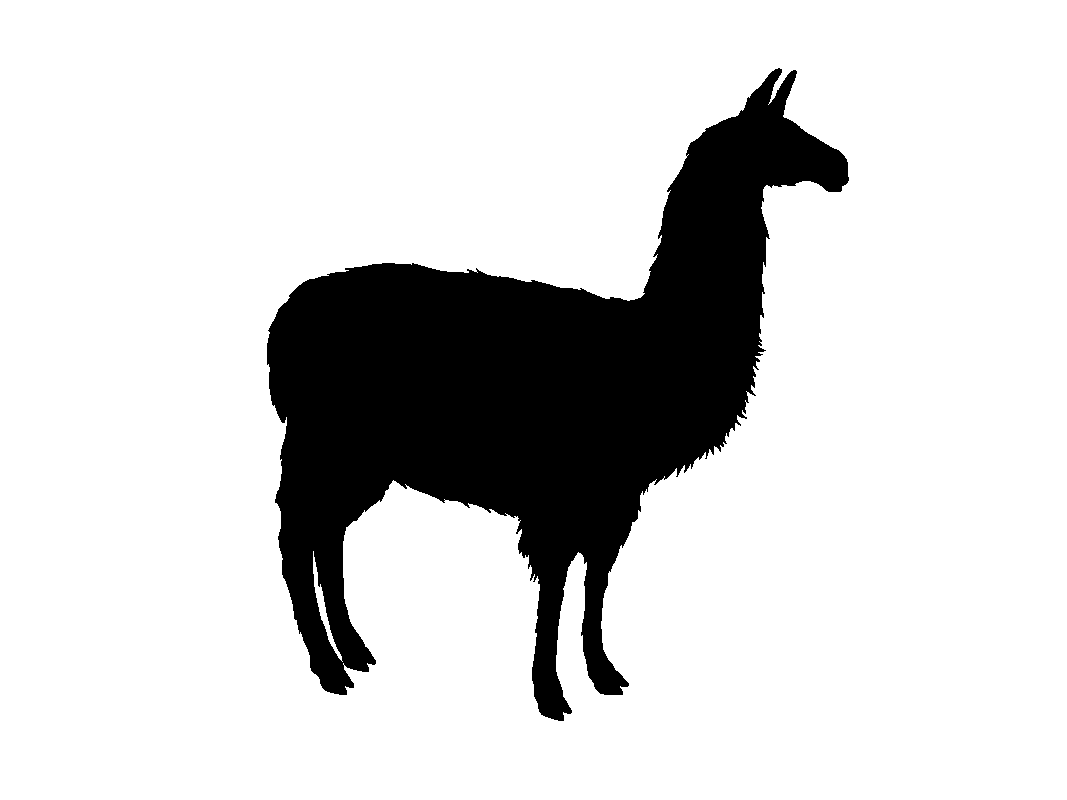
\includegraphics[width=#1]{../llama.pdf}}
\newcommand\llitem{\item[\raisebox{-0.15em}{\llama{1.2em}}]}

\begin{lemma}[Equivalence of Aborts]
	\label{lem:equiv}
	Let:
	\begin{itemize}
		\item $\tiiat{\alpha}$ be an HTM begin operation,
		\item $\tiiat{\beta_1}\dots\tiiat{\beta_n}$ be the transaction body (with $\beta_n$ the HTM end call),
		\item $\tiiat{\phi_1}\dots\tiiat{\phi_m}$ be the failure path, and
		\item $\tiiat{\omega_1}\dots\tiiat{\omega_l}$ be the subsequent code executed unconditionally.%
			\footnote{Arbitrary code may not be structured to distinguish these as nicely as in our examples;
			e.g., more code may exist in the success branch after {\tt \_xend()};
			such would be considered part of $\omega$ here.}
	\end{itemize}
	Then, for any interleaving prefix%
	\footnote{Without loss of generality: for any number of other threads \tjj/\tkk,
	and for any number of thread switches away from \tii during the transaction.}
	\[
		\tiiat{\alpha},\tiiat{\beta_1}\dots\tiiat{\beta_b},
		\tjjat{\gamma_1}\dots\tjjat{\gamma_j},
		\tkkat{\kappa_1}\dots\tkkat{\kappa_k},
		\tiiat{\beta_{b+1}} % $\dots\tiiat{\beta_{n-1}}$ -- excluded bc might abort
	\]
	with $b<n$, $j \ne i$, $k \ne i$, etc., either:
	\begin{enumerate}
		\item $\tiiat{\alpha},\tjjat{\gamma_1}\dots\tjjat{\gamma_j},\tkkat{\kappa_1}\dots\tkkat{\kappa_k},\tiiat{\phi_1}\dots$
			(conflicting case), or
		\item $\tiiat{\alpha},\tiiat{\beta_1}\dots\tiiat{\beta_b}\dots\tiiat{\beta_n},\tjjat{\gamma_1}\dots\tjjat{\gamma_j},\tkkat{\kappa_1}\dots\tkkat{\kappa_k}$
			(independent case)
	\end{enumerate}
	exists and is observationally equivalent.
\end{lemma}

\begin{proof}
	We case on whether the operations by \tjj and/or \tkk have any memory conflicts (read/write or write/write)
	with $\tiiat{\beta_1}\dots\tiiat{\beta_n}$.
	If so, then the hardware will abort \tii's transaction, discarding the effects of $\tiiat{\beta_1}\dots\tiiat{\beta_n}$
	and jumping to $\tiiat{\phi_1}$,
	satisfying case 1.
	Otherwise, by DPOR's definition of transition dependence \cite{dpor}, %,landslide-phdthesis},
	$\tiiat{\beta_{b+1}}\dots\tiiat{\beta_n}$ is independent with the transitions of \tjj and \tkk,
	may be successfully executed until transaction commit,
	and reordering them produces an equivalent interleaving,
	satisfying case 2.
\end{proof}

The second part of our claim follows naturally.

\begin{theorem}[Atomicity of Transactions]
	\label{thm:atom}
	For any state space $S$ of a transactionally-concurrent program,
	an equivalent state space exists in which all transactions are either executed atomically or aborted immediately.
\end{theorem}

\begin{proof}
	For every $I \in S$ with $\tiiat{\alpha},\tiiat{\beta_1}\dots\tiiat{\beta_b},$ $\tjjat{\dots},\tkkat{\dots},\tiiat{\beta_{b+1}} \in I$,
	apply Lemma~\ref{lem:equiv} to obtain an equivalent interleaving $I'$ satisfying the theorem condition.
	The resulting $S'$ can then be MCed without ever simulating HTM rollbacks.
\end{proof}

\subsection{Memory Access Analysis}

Next, we address the memory accesses within transactions with regard to data-race analysis.
From Theorem~\ref{thm:atom} we have that the body of all transactions may be executed atomically within the MC environment.
While they may interleave between other non-transactional sequences,
no other operations (whether transactional or not) will interrupt them.
We claim this level of atomicity is equivalent to that provided by a global lock,
and hence abstracting it as such in Landslide's data-race analysis is sound.

Let $\tiiat{\mu},\tjjat{\nu}$ be a pair of memory accesses to the same address, at least one a write,
in some transactional execution $I$ normalized under Lemma~\ref{lem:equiv}.
Then let $\mathsf{lockify}_m(\tkkat{L})$ denote a function over instructions in $I$,
which replaces $\tkkat{L}$ with $\tkkat{\mathsf{lock}(m)}$ if $L$ is a successful HTM begin,
with a no-op if $L$ is a transaction abort,
or with $\tkkat{\mathsf{unlock}(m)}$ if $L$ is an HTM end,
or no replacement otherwise.
Finally, let $I' = \exists m. \mathsf{lockify}_m(I)$,
the execution with the boundaries of all successful transactions replaced by an abstract global lock.
Lemma~\ref{lem:equiv} guarantees mutual exclusion of $m$.

\begin{theorem}[Transactions are a Global Lock]
	$\tiiat{\mu},\tjjat{\nu}$ is a data race in $I$ iff it is a data race in $I'$.
\end{theorem}

\begin{proof}
We prove one case for each variant definiton for data races supported in Landslide \cite{quicksand}.
For each, we semiformally state what it means to race in an execution with synchronizing HTM instructions.

\begin{itemize}
	\item {\bf Limited Happens-Before.}
		%Under this definition,
		To race in $I$ they must be reorderable at instruction granularity,
		at least one with a thread switch immediately before or after.
		\cite{tsan,hybriddatarace}.
		\begin{itemize}
			\llitem $I \Rightarrow I'$:
				If $\tiiat{\mu},\tjjat{\nu}$ race in $I$,
				then they cannot both be in successful transactions,
				or else placing \tiiat{\mu} within the boundaries of \tjjat{\nu}'s transaction
				would cause the latter to abort, invalidating \tjjat{\nu}, or vice versa.
				Hence they will not both hold $m$ in $I'$.
				Otherwise their lock-sets and DPOR dependence relation remain unchanged.
			\llitem $I' \Rightarrow I$:
				If $\tiiat{\mu},\tjjat{\nu}$ race in $I'$,
				both corresponding threads cannot hold $m$;
				WLOG let $\tii$ not hold $m$ during $\tiiat{\mu}$.
				Then in $I$, $\tiiat{\mu}$ is not in a transaction.
				With the remainder of their lock-sets still disjoint,
				and still not DPOR-dependent, $\tjjat{\nu}$ (or its containing transaction)
				can then be reordered directly before or after $\tiiat{\mu}$.
		\end{itemize}
	\item {\bf Pure Happens-Before.}
		WLOG fix $\tiiat{\mu} \prec \tjjat{\nu} \in I$.
		Then to race in $I$ there must be no pair of synchronizing instructions
		$\tiiat{\epsilon}$ (a release edge) and $\tjjat{\chi}$ (an acquire edge) such that
		\[
			\tiiat{\mu} \prec \tiiat{\epsilon} \prec \tjjat{\chi} \prec \tjjat{\nu} \in I
		\]
		to update the vector clock epoch between \tiiat{\mu} and \tjjat{\nu} \cite{djit,fasttrack}.
		\begin{itemize}
			\llitem $I \Rightarrow I'$:
				If $\tiiat{\mu},\tjjat{\nu}$ race in $I$,
				then they cannot both be in successful transactions,
				or else Lemma~\ref{lem:equiv} normalization would provide
				the corresponding HTM end and begin for $\tiiat{\epsilon}$ and $\tjjat{\chi}$ respectively.
				Hence there will be no unlock/lock pair on $m$ in $I'$ to satisfy the above sequence.
			\llitem $I' \Rightarrow I$:
				If $\tiiat{\mu},\tjjat{\nu}$ race in $I'$,
				then they cannot both hold $m$,
				or else $\mathsf{lockify}_m$ would provide the corresponding
				unlock and lock for $\tiiat{\epsilon}$ and $\tjjat{\chi}$ respectively.
				Hence there will be no HTM end/begin pair in $I$ to satisfy the above sequence.
		\end{itemize}
		%In both cases $I$ and $I'$ otherwise have the same synchronizing instructions.
\end{itemize}
Hence, data-race analysis is sound when transaction boundaries are replaced by an abstract global lock.
\end{proof}


\end{document}
